\tightsection{The GO Prediction Algorithm}
\label{sec:prediction}
In this section, we present a practical algorithm that addresses the challenges presented in \Section~\ref{subsec:aggregation}. We show that this algorithm makes similar predicted quality to optimal AC, and show that the resulting prediction error is much closer to the lower bound introduced in \Section~\ref{subsec:lowerbound} compared with representative strawman algorithms.
%\jc{We don't discuss temporal attribute aggregation. Need to say something about that. In all experiments, I used 30 minutes time window}

This section begins with the basic framework of prediction algorithm (\Section~\ref{subsec:basic}). We then present two techniques and their empirical evaluation to address the limitations of the basic algorithm so as to improve the prediction accuracy (\Section~\ref{subsec:acs}, \Section~\ref{subsec:sudo}). Finally, \Section~\ref{subsec:minieval} compares the prediction error of GO with that of strawman algorithms (where ACs are not dynamically chosen) as well as the lower bound.


\tightsubsection{Basic Algorithm}
\label{subsec:basic}
The tradeoff between estimation error and bias via aggregation naturally leads us to consider a class of algorithms that compute average quality outcomes for groups of sessions under different attribute sets, and then {\it dynamically} choose the attribute set that seems to work well for a given session. 
%However, it is difficult to find a globally best AC, it is useful to hedge our bets by taking a weighted combination of averages. \xil{did we prove this?}
We propse the following basic structure for the algorithm. The algorithm chooses a set of ACs offline (called {\it ACS}), which can consist of all possible ACs $G$, i.e., full ACS, or a subset of them. 
We explain why full ACS is not the best choice and how we select the ACS in \Section~\ref{subsec:acs}. When an ACS is chosen offline, the algorithm starts collecting quality metrics for all the identical groups of each AC in the ACS 
(of which Figure~\ref{fig:example-optimal-ac} gives an example when ACS consists of all ACs of the three attributes). Based on the quality metrics collected, each identical group will be given a weight so that the weights reflect statistical properties of the identical groups and are thus updated when new quality samples are collected.
Finally, when receiving a session $s$ under prediction, for $g_i\in G$, let $w_i$ be the weight given to the identical group of $g_i$ that includes $s$, and the mean quality of this identical group is $p_i$,
the prediction is an weighted sum of the mean quality of each group, $p=\frac{1}{\sum_{g_i\in G} w_i}\sum_{g_i\in G} w_ip_i$.

The next question then becomes how to design a weighting scheme to balance between estimation error and bias to minimize overall prediction error. 
%Intuitively, we would like to use larger $w_i$ for finer granular groups if they do not have high estimation error. 

George et al~\cite{george2008value} consider this problem and the proposed prediction algorithm WIMSE, for Weighted Inverse Mean Squared Error.  Inverse-mean-squared-error weighting has the following desirable property: If the mean quality $p_i$ of each group is statistically independent, then the resulting prediction is an optimal estimator in the sense that it has the minimal overall prediction error among all samples drawn from the same distribution~\cite{george2008value}.
While the algorithm achieves optimality under some assumption and George et al have found that WIMSE can nevertheless work well in most cases, there are two problems with this algorithm, which we will try to address in the following sections.
\begin{packeditemize}
	\item {\bf ACS selection:} In our setting the $p_i$ values are based on overlapping data and are therefore not always independent. For example, if a coarser-grained group is generated by aggregating together finer-grained groups, both the coarser and finer groups will receive similar weights as their mean qualities are dependent; including both ACs doubles the weight of the corresponding groups for no principled reason. We present a algorithm to efficiently select an ACS that performs empirically the best with WIMSE in~\Section~\ref{subsec:acs}.
	\item {\bf Non-normal distribution:}  WIMSE becomes challenging if samples in fine-grained groups follow a non-normal distribution and very sparse. Especially when predicting for buffering ratio or start failure, where the quality of most samples are zero (i.e., no buffering happened or video successfully started), it is very likely to have a few samples with the same value and thus, lead to large bias.  We address this by borrowing the idea of pseudocount prior in~\Section~\ref{subsec:sudo}.
\end{packeditemize}

\tightsubsection{Efficient ACS Selection}
\label{subsec:acs}
The key for WIMSE to work in our use case (with the power set of possible ACs, or in total, $2^k$ in case of $k$ attributes) is to select the right ACS.
The most straightforward approach of using full ACS does not work well not only because the independence assumption is dramatically violated, 
but also the computational costs of WIMSE grow exponentially with the more attributes.

To pick the best ACS, we take a data-driven approach, where we split our data sets into training and testing data sets. 
Then, the best ACS is the one that gives the minimal overall prediction error over the test set using WIMSE with this ACS. 
In this context, we still have two decisions to make: searching complexity (greedy vs. exhaustive search) and granular of selection.


\myparatight{Greedy vs. exhaustive search\jc{This part should be removed or downplayed}} One problem with the exhaustively search is that even in offline analysis, the potential space to search for the best ACS is too huge (with $k$ attributes, there will be $2^k$ ACs, and in total $2^{2^k}$ ACSes). Instead, we examine a greedy algorithm which finds a good ACS in $O(2^k)$ steps, called {\it greedy search}, and compare it against exhaustive search result for $k=3$ attributes on which exhaustive search is possible. The greedy algorithm incrementally adds to an existing ACS one AC at a time which reduces the prediction error with most magnitude.
We use our dataset and three attributes of $ASN$, $ConnectionType$ and $OS$ in addition to $Initial CDN$ and $Initial Bitrate$ which are by default selected.
Table~\ref{tab:greedy-exhaustive} compares the ACS selected by two methods. It shows that in most cases ($\sim$90\% of minutes) the ACS selected by the two methods are identical and that even when different, they are still very similar\footnote{Jaccard index between two sets $A,B$ is $\frac{|A\cap B|}{|A\cup B|}$}. This means that a near-optimal ACS can be identified in tractable steps.
\xil{a natural question is what if $k>3$, we need to justify why we do not do that experiment. also, since this is offline, we need to justify the contribution here (such as it takes how many days to do exhaustive search on 10 attributes).}

\begin{table}[t]
\begin{center}
\begin{small}
\begin{tabular}{p{2.2cm}|p{1.1cm}|p{1.1cm}|p{1.1cm}|p{1.1cm}}
		& BufRatio & Bitrate & JoinTime & StartFailure\\ \hline 
Frac. of same ACS & 0.93 & 0.98 & 0.88 & 0.97 \\
Mean of Jaccard & 0.8 & 0.83 & 0.92 & 0.83 \\
\end{tabular}
\end{small}
\end{center}
\tightcaption{Greedy vs. exhaustive search: Fraction of times when greedy search gives the same ACS as exhaustive search does, and the Jaccard similarity index between ACSes chosen by the two methods when they are different. }
\label{tab:greedy-exhaustive}
\end{table}

\myparatight{Granular of selection} The ACS selection could be to find one ACS that produces best overall prediction accuracy called global ACS, or to find one ACS for each (non-overlapping) partition that gives best prediction individually, called per-group ACS. 
\xil{need an example}
It is hard to theoretically justify which one is better. However, we use our dataset to demonstrate that global ACS is sufficiently good and sometimes better than per-group ACS.
Figure~\ref{fig:global-acs} shows the CDF of prediction error on buffering ratio on each session under prediction and use it to compare global ACS and per-group ACS. For per-group ACS, we consider the finest group (i.e., the selected ACS can vary across the finest groups). It shows that they perform similarly and the global ACS performs even slightly better, possibly because per-finest-group ACS has side-effect of overfitting.
\xil{again we need to justify more because this is offline. a related question is what if things change?}

\begin{figure}[h!]
\centering
 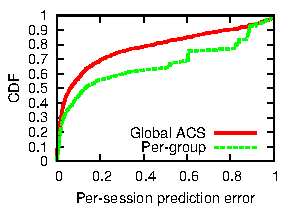
\includegraphics[width=0.3\textwidth] {figures/newfig/example-granular-metric0-new.pdf}
\tightcaption{Comparison of different granular of selection. Per-group ACS selection picks the best ACS in each finest group using history data. Somewhat suprisingly, choosing ACS for each finest group will increase prediction error due to overfitting.}
\label{fig:global-acs}
\end{figure}

To conclude, based on the above empirical analysis, GO's ACS selection searches for best global ACS using greedy algorithm. 

\tightsubsection{Handling Non-Normal Distribution}
\label{subsec:sudo}
The WIMSE algorithm assumes that bias and variance can be computed exactly, while in practice variance cannot be estimated accurately when groups are very small and the sample distribution does not follow normal distribution. For instance, it is very likely to have all samples in a group with the same values and prediction based on this information will be greatly biased and even worse, WIMSE will treat this group as with zero variance. This is a particularly serious problem for video quality metrics such as buffering ratio and start failure where value of zero is usually dominant.
To alleviate this, we use a simple idea from Bayesian statistics~\cite{}\jc{Henry, give a pointer}: We incorporate a prior distribution on quality outcomes within each group.  This amounts to adding a few fake ``pseudocount'' observations to each group.  Empirically, we see an reduction of at most 5.6\% in prediction error in buffering ratio and 4.5\% in start failure.

\comment{
\begin{figure}[h!]
\centering
 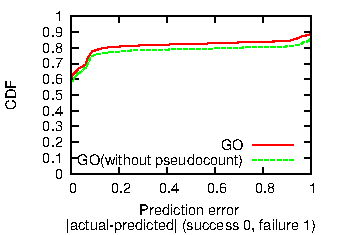
\includegraphics[width=0.4\textwidth] {figures/prediction-comparisons/example-pcount-metric3.pdf}
\tightcaption{GO with pseudocount vs. without pseudocount (considerd quality metric is average bitrate).}
\label{fig:sudocount}
\end{figure}
}

\begin{figure*}[t!]
\centering
\subfigure[Buffering ratio (\%)]
{
        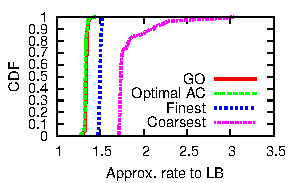
\includegraphics[width=0.25\textwidth]{figures/newfig/example-fig-cdf-all-metricId0.pdf}
}
\hspace{-0.6cm}
\subfigure[Average bitrate (Kbps)]
{
        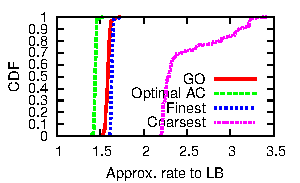
\includegraphics[width=0.25\textwidth]{figures/newfig/example-fig-cdf-all-metricId1.pdf}
}
\hspace{-0.6cm}
\subfigure[Join time (ms)]
{
        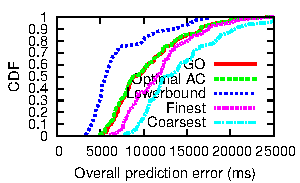
\includegraphics[width=0.25\textwidth]{figures/newfig/example-fig-cdf-all-metricId2.pdf}
}
\hspace{-0.6cm}
\subfigure[Start failure (\%)]
{
        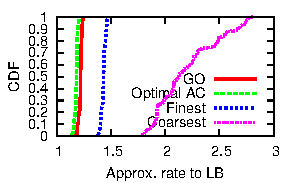
\includegraphics[width=0.25\textwidth]{figures/newfig/example-fig-cdf-all-metricId3.pdf}
}
\tightcaption{Comparison between GO with two oracle approaches (lower bound and optimal AC) and two strawman approaches (static finest/coarsest AC).}
\label{fig:compare-to-naive}
\end{figure*}

\tightsubsection{Evaluation of Prediction Error}
\label{subsec:minieval}

To conclude the section, we compare GO (with ACS selection and pseudocount prior) against two oracle approaches -- the lower bound (\Section~\ref{subsec:lowerbound}) and the optimal AC (\Section~\ref{subsec:aggregation}).  Recall that the optimal AC reflects the best possible prediction using an appropriate AC of historical data if quality informaton of sessions under prediction is known. The lower bound represents the best possible prediction in theory with no constraint on the way we use historical data. Figure~\ref{fig:compare-to-naive} shows the distribution of overall prediction error at each minute using different methods. It suggests that GO performs very similarly to optimal AC (e.g., with a difference of 80 Kbps in average bitrate) and close to the lower bound (e.g., a difference of 300 Kbps in average bitrate). 

To put this prediction accuracy into context, we also consider two strawman prediction algorithms that do not use adaptive degree of aggregation.
\begin{packeditemize}
	\item Coarsest AC: Predict using average of each CDN and bitrate combination: picking the decision that is globally best (i.e., no client-side spatial partition)
	\item Finest AC: Predict using average of the finest group that has any data.
\end{packeditemize}

All these results indicate that GO performs better than both strawman, with reduction in prediction accuracy of almost 25+\% from coarsest AC and 1-10\% from finest AC all four metrics. This confirms the observation in \Section~\ref{subsec:aggregation} that the best level of aggregation is often dynamic and in between the coarsest and finest aggregation.


Finally, we look into the result in more details. Figure~\ref{fig:compare-partition} partitions the results by different Sites and picks the largest 3 Sites in which we compare GO's prediction error in buffering ratio and average bitrate with the strawman (Coarsest) as well as the lower bound. As shown, with the lower bound varying across different Site, GO can always achieve closer-to-optimal prediction accuracy (i.e., low overall prediction error) than the strawman.

\begin{figure}[h!]
\centering
\subfigure[Buffering ratio]
{
        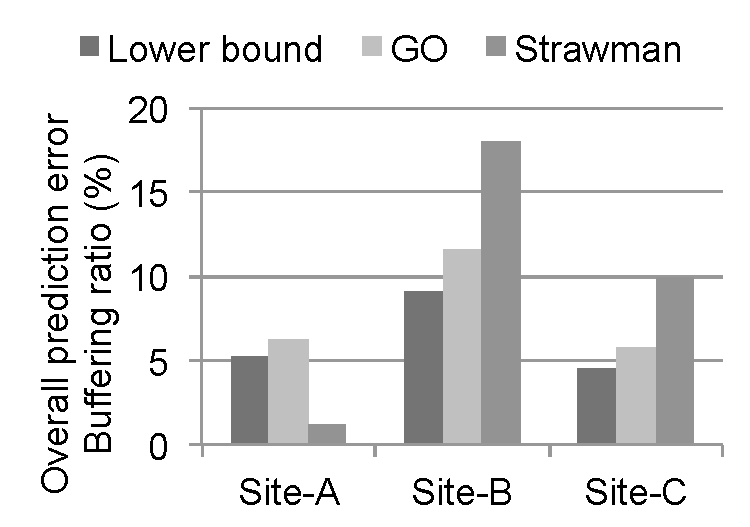
\includegraphics[width=0.24\textwidth]{figures/newfig/bar-compare-bufratio.pdf}
}
\hspace{-0.6cm}
\subfigure[Average bitrate]
{
        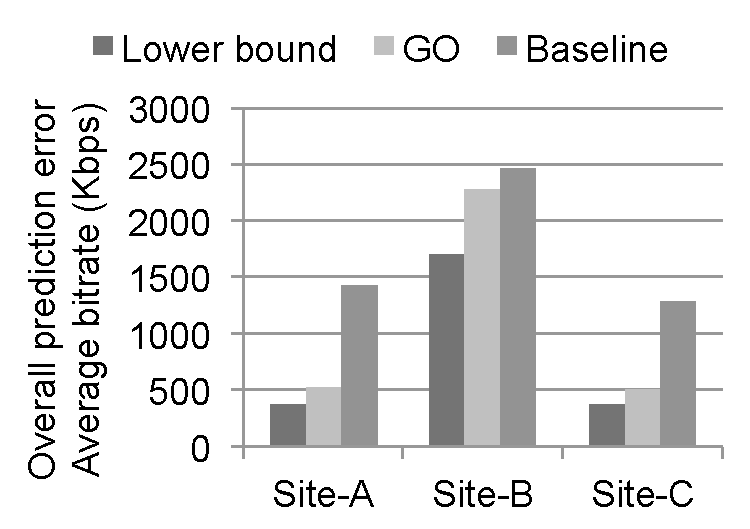
\includegraphics[width=0.24\textwidth]{figures/newfig/bar-compare-bitrate.pdf}
}
\tightcaption{Comparison of prediction error between GO, lower bound and strawman (coarsest AC) in different Sites.}
\label{fig:compare-partition}
\end{figure}


%% content below may be put into discussion section
\comment{
\tightsubsection{Interactions between decisions\jc{Move to discussion}}
The reader may be bothered by a simplifying assumption implicit in our characterization of the causes of prediction error.  If we allocated all traffic to a single CDN, its performance might degrade, but our session-wise prediction does not capture that.  We might instead want to know the following: Given a set of decisions about sessions (say, all the sessions we observe in a 1-hour interval), what is the predicted performance for that set of sessions?  We do not wish to say that such a question is impossible to answer, but rather point out some difficulties in answering it, and some reasons why it is less critical to answer it than it may appear.

Joint prediction is statistically difficult because existing statistical prediction algorithms typically assume the performance of training examples are independent and experience identical randomness (i.e. they are IID).  We observe very few IID instances of whole sets of sessions; in our example, we observe only one per 1-hour interval.  It is possible to model explicitly the dependence of each session’s performance on the set of joint decisions, but this requires modeling choices that we may not make well, and such models are typically computationally expensive to learn. \fillme

If conditions change slowly enough, the independence assumption is not so bad.
The rate of change of CDN allocations is naturally limited for our problem by the rate of session arrivals, since we choose CDNs only at the beginning of each session.  Spikes in the rate of new sessions are not typically high enough to necessitate special handling.  \henry{Need some data and experiments for this.  Davis or Florin have done some of the experiments, I think.}


\tightsubsection{Alternative approaches\jc{Move to discussion}}
The reader should not leave with the impression that the algorithm described above is the only possible one for predicting video quality, or even the best.  The scope of this paper is merely to establish a reasonable approach and show that it results in improvements.  Other possible approaches might include:
\begin{packedenumerate}
  \item \emph{Linear regression:} After encoding categorical attributes as binary features, simple linear regression can be applied to predict quality outcomes.  Temporal attributes can be passed through nonlinear functions to achieve reasonable time-series prediction.  Interaction terms (e.g. the indicator for a session coming from ASN $100$ multiplied by the indicator for the session having Object ``foo'') can simulate attribute combinations, at the cost of a combinatorial explosion in the size of the learned model.  However, recent developments in optimization for $\ell_1$-regularized linear regression allow models to be learned quickly online while providing the guarantee that the learned model is \emph{sparse}, i.e. that only a few important features are selected for inclusion in the model and the rest can be safely dropped.  See \cite{duchi2010composite} for one example of work that could enable this technique.  One downside is that linear models are harder to interpret than a model based on averaging group averages.
  \item \emph{Hierarchical Bayesian modeling:} In this approach, groups are placed in the natural tree, and each is associated with a probability distribution over quality outcomes, such as a Gaussian distribution.  Each group inherits information from the distribution of its parent group in the form of a prior.  Such models potentially deal very naturally with data sparsity and with dependence among sessions \cite{gelman2003bayesian}, but learning them from data is often computationally intractable.
\end{packedenumerate}
}
